\chapter{Návrh  riešenia}

Mojim návrhom je implementácia systému, ktorá umožní používateľovi prípravu pred prezentáciou a taktiež aj spracovanie už existujúceho záznamu prezentácie. Rozhodol som sa využiť \textbf{mobilné zariadenia}, ktoré dnes má takmer každý človek a sú vybavené vstavanou kamerou. Z týchto zariadení vytvorí používateľ video, ktoré následne odošle pomocou mobilnej aplikácie na aplikačný server, ktorý prezentáciu zanalyzuje a poskytne spätnú väzbu. Moja aplikácia teda bude fungovať na \textbf{záznamoch} a nie na živom prenose. Aplikácie bude ponúkať dve základné funkcie a to:
\begin{itemize}
    \item Trénovanie konkrétneho javu
    \item Celková analýza prezentácie
\end{itemize}
Pri \textbf{trénovaní konkrétneho javu} si používateľ zvolí jednu z možností, na čo sa chce zamerať a následne natočí video, ktoré mu systém následne zhodnotí. Príkladom je, že používateľ sa chce naučiť správne využívať očný kontakt, tak moje riešenie mu dovolí umiestniť zariadenie dostatočne ďaleko a následne natočiť video a odoslať pre spracovanie. V tomto móde systém spúšta iba jeden druh detekcie a sústredí sa naň.

\textbf{Celková analýza prezentácie} poskytuje spätnú väzbu vo všetkých oblastiach prezentácie. V prípade, že systém nevie spoľahlivo určiť niektorú z funkcií, oznámi to používateľovi a tento jav nedetekuje. Napríklad ak nevie kamera zachytiť zápästia používateľa z dôvodu, že je ho ruky su mimo kameru, upozorní ho na to.

\section{Špecifikácia požiadaviek}
Pred samotnou implementáciou som definoval niekoľko funkčných požiadaviek, ktoré by aplikácia mala spĺňať. Pri rozhodovaní, ktoré údaje budem detekovať som sa odrážal od môjho výskumua porovnaní existujúcich riešení, ktorý bol bližšie popísaný v sekcii analýza problematiky.
\begin{itemize}
    \item \textbf{Detekcia očného kontaktu}: Systém musí vedieť rozpoznať, či sa prezentujúci pozerá smerom do publika a nie je k nemu otočený chrbtom. Pre detekciu tohto javu sa využije viditeľnosť očí voči kamere, ktorá bude pred prezentujúcim.
    \item \textbf{Detekcia pohybu bokov}: Systém musí vedieť detekovať negatívny jav, nazývaný ako tancovanie (pohyb bokov zo strany na stranu). Detekcia bude počítaná akceleráciou stredu medzi bokmi, a bude detekovať kývanie z prava do ľava a z predu do zadu.
    \item \textbf{Detekcia pohybov rúk}: Systém musí vedieť detekovať nedostatočné pohyby rúk v prezentácii. Taktiež počítaná sledovaním akcelerácie rúk. Zároveň bude systém sledovať opakujúce sa gestá.
    \item \textbf{Detekcia monotónnosti}: Systém musí vedieť detekovať monotónny hlas. Monotónnosť hlasu je definovaná ako konštantný tón hlasu počas prezentácie. Bude sa teda sledovať zmena tónu hlasu.
    \item \textbf{Detekcia hlasitosti}: Systém musí vedieť detekovať nízku hlasitosť prezentujúceho.
    \item \textbf{Detekcia výplňových slov}: Systém musí vedieť detekovať výplňové slová.
    \item \textbf{Detekcia kritických bodov zmien}: Systém musí pre relevantné kritériá uvedené vyššie definovať kritické body, kedy sa drasticky zmenil doterajší priebeh. Ide napríklad o definovanie hranice, kedy prezentujúci prestal náhle využívať všetky pohyby rúk, alebo že v prvej minúte prezentácie využíval veľké množstvo výplňových slov.
\end{itemize}

\newpage

\section{Architektúra riešenia}
Nakoľko som počas analýzy zistil, že nevhodných javov ktoré je možné detekovať je veľke množstvo, navrhujem mikroslužbovou architektúru, kde každá mikroslužba bude detekovať skupinu súvisiacich negatívnych javov. Dôvodom použitia mikroslužieb je ich vlastnosť jednoduchého nasadzovania, ktorá môže byť využitá pri pridávaní nových detekcií. Zároveň mikroslužbová architektúra umožnuje technologickú voľnosť, ktorá by sa v prípade rozširovania mojej práce zišla. Všeobecná architektúra by obsahovala:
\begin{itemize}
    \item Mobilnú aplikáciu
    \item API Gateway
    \item Mikroslužba pre analýzu videa
    \item Mikroslužby pre detekciu javov
    \item Databáza
\end{itemize}


Pre pochopenie som vytvoril sekvenčný diagram, ktorý znázorňuje interakciu používateľa so systémom, kde chce detekovať konkrétne pohyb rúk.

\begin{figure}[H]
\begin{centering}
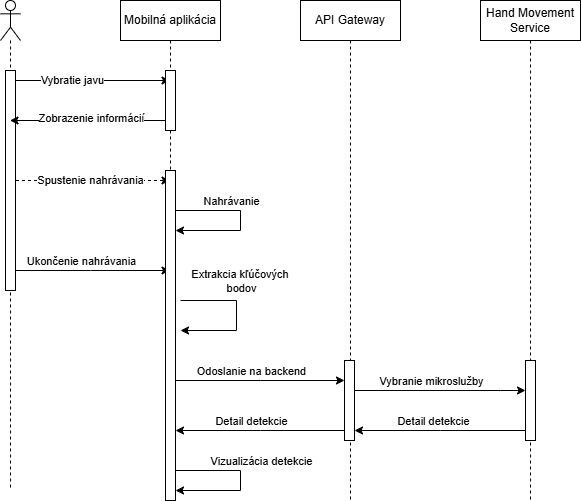
\includegraphics[width=\textwidth, height=12cm]{assets/images/implementation/detekciaKonkretne.png}
\par\end{centering}
\caption{Príklad interakcie s aplikáciou v móde trénovania konkrétneho javu \label{fig:sequenceSingleDetect}}
\end{figure}

Pri detekcii všetkých negatívnych javov pribúda ešte mediator, ktorý po nahratí videa spustí detekciu na všetkých mikroslužbách a vytvorí komplexnú odpoveď so všetkými údajmi.

\begin{figure}[H]
\begin{centering}
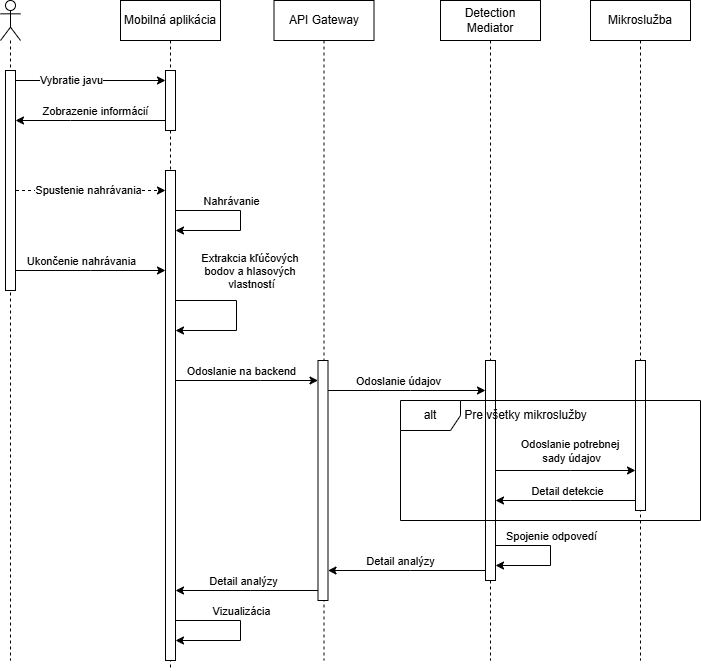
\includegraphics[width=\textwidth]{assets/images/implementation/detectionAll.png}
\par\end{centering}
\caption{Príklad interakcie s aplikáciou v móde celkovej analýzy\label{fig:sequenceAllDetect}}
\end{figure}

\newpage
Celkový diagram systému bude teda nasledovný:

\begin{figure}[H]
\begin{centering}
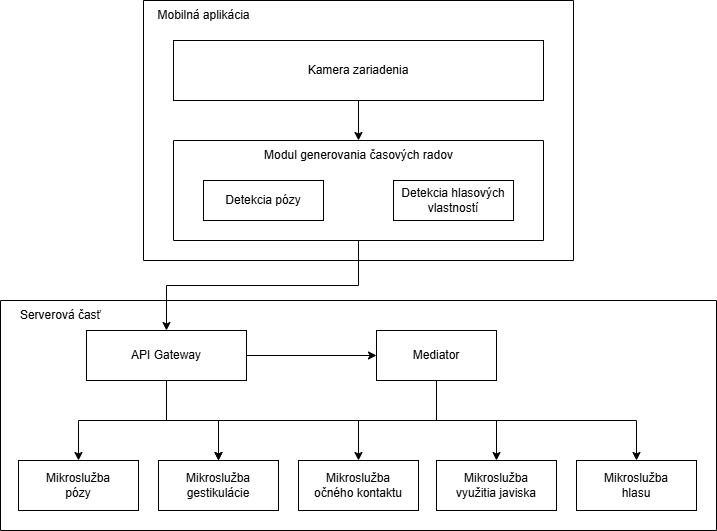
\includegraphics[width=\textwidth]{assets/images/implementation/architecture.png}
\par\end{centering}
\caption{Architektúra aplikácie \label{fig:sequenceAllDetect}}
\end{figure}

Diatram je rozdelený na mobilnú aplikáciu a serverovú časť.

\textbf{Mobilná aplikácia} má za úlohu vytvorenie videa a vytvorenie časových radov pre video. Tieto údaje následne posielá na \textbf{API Gateway}, ktorý slúži ako proxy, ktoré posunie iba podstatné údaje do \textbf{mikroslužby}, ktorá detekuje potrebné vlastnosti. Taktiež je zobrazený aj \textbf{mediator}, ktorý sa bude využívať pri detekcii všetkých javov.

\subsection{Použité technológie}

Z hľadiska využitých technológií chcem pre mobilnú aplikáciu využiť framework \textbf{Flutter}, čim zabezpečím dostupnosť aplikácie pre hlavné platformy na mobilných zariadeniach. Pre serverovú časť chcem použiť framework \textbf{django}, ktorý je využíva programovací jazyk Python. Tento jazyk je štandardným jazykom pre strojové učenie a disponuje veľkým množstvom knižníc pre analýzu časových radov. Pre detekciu kľúčových bodov polohy využijem \textbf{Google ML Kit} a konkrétne \textbf{pose detection}, ktorá mi poskytne všetky potrebné kľúčové body. Nasledujúci obrázok zobrazuje všetky body, ktoré táto knižnica vie detekovať\cite{googleMLKit}.

\begin{figure}[H]
\begin{centering}
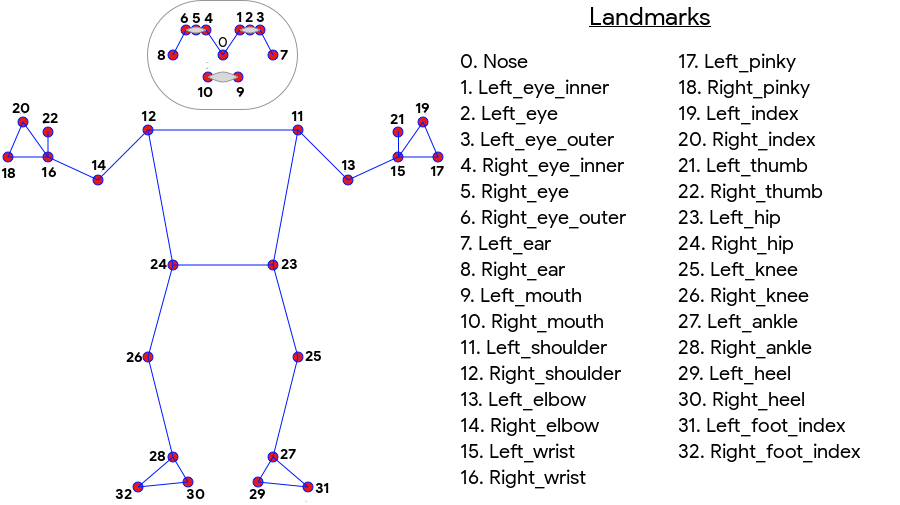
\includegraphics[width=\textwidth]{assets/images/implementation/poseDetecion.png}
\par\end{centering}
\caption{Kľúčové body detekované Google ML kitom \label{fig:sequenceAllDetect}}
\end{figure}